\chapter{From signals to images}
\label{chapter:two}
%Contiene el método y el enfoque.

%Mental Chrometry and averaging 
%https://www.ncbi.nlm.nih.gov/pmc/articles/PMC548951/

A regular practice in image processing is to analyze images as bidimensional signals.  In this Thesis the opposite is done and signals are studied by how they are represented on images. This chapter describes the procedure to plot an image from the digital EEG signal.  This image is used to extract a features which represents the waveform, the structure of the signal on a plot.  By analyzing these features, we hypothesize that the underlying cognitive process can be detected and it can be used to implement a brain-computer communication device.

\section{Electroencephalographic Plotting}

The plotting of the EEG is intrinsically mixed with the nuisances of the electroencephalography itself.  Plotting proceed by using a chart recorded with a single pen~\cite{Jestico1977}.   Voltages are represented on a vertical axis while time is represented on the horizontal axis, in a Cartesian arrangement.  The most salient characteristics of a plot are:

\begin{enumerate}
\item Sensitivity: also termed gain due the amplification procedure.  Its units are $ \frac{mV}{mm}$.  In the digital form, it is $\frac{\mu V}{pixel}$.
\item Epoch/Paper speed: the time span that is represented in a single screen.  For paper strips it is usually $10s$.  In its digital counterpart is $ \frac{w}{pixel}$ with $w$ being the length in seconds of the signal segment.
\end{enumerate}

Additionally, on analog plotting montage is essential, while digital plotting allows flexible montage configuration from software.  Montage can be monopolar or bipolar.  On monopolar montages each electrode obtains the potential difference against a common reference. With bipolar montages, electrodes are paired, eventually in chained configurations, and the potential difference is obtained between each pair of electrodes~\cite{EEGIntro}.

%Logarithmic plotting, montage, calibration (cite Electroencphalograpy for empilepsy society)

\begin{story}[Neuroimaging]
With the advent of digital computers and the digital revolution, plotting has became imaging.  Medical imaging is defined as the making of a visual representation of an organ with a detector or sensor.  However, the concept has extended and brain imaging modalities is  synonym of brain measuring devices.  Neuroimaging~\cite{Freeman2013} entails image mapping activity or structure to neuroanatomical regions.  There are currently three categories of neuroimaging: \textit{structural} which includes Computed Tomography (CT), Magnetic Resonance Imaging (MRI) and Diffusion Tensor Imaging (DTI), \textit{functional}, which encompass EEG, MEG, fMRI, PET, Single Positron Emission Computed Tomography (SPECT), NIRS and \textit{chemical} which involves special dyes which are sensible to neuron firing.  Indeed, analyzing image plots is a form of brain imaging.
\end{story}

% Brain imaging modalities.

\section{Signal to Image transformation}

The EEG signal is represented by

\begin{equation}
x(n,c)
\label{eq:eegdefinition}
\end{equation}

\noindent where $n$ is the index of sample points digitalized at sampling frequency $\gls{Fs}$.  This is a multichannel signal, for $c$ varying between  $1 \leq c \leq \gls{C}$.  Each one of this channels is assigned a name according to the 10-20 international system (see Figure \ref{fig:electrodelocations}), and there are $\gls{C}$ available channels. The sample index $n$ varies between $1$ and $\gls{N}$.  The span of the signal $\lambda$ is the length in milliseconds of the waveform under study. 

The length of segment $\gls{N}$ in sample point units, the sampling frequency $\gls{Fs}$ in \si{\hertz} and the segment length $\gls{w}$ in seconds are related by

\begin{equation}
N = \left\lfloor F_s \; w \right\rfloor.
\label{eq:segmentlength}
\end{equation}

Additionally the signal can be scaled on amplitude by the scale factor $\gls{gamma}$ or in time by the factor $\gls{gammat}$.  The  $\gls{gammat}$ parameter can also be used to convert from time to sample point index by

\begin{equation}
n = \left\lfloor F_s \; t \right\rfloor \; \gls{gammat}  .
\label{eq:samplepointconversion}
\end{equation}

\vspace{3pt}

To extract features from an image, it should be first constructed.  The straightforward way to do it, replicating the analog or digital EEG plotting, is to draw a line on a contrast background.  This line represents the voltage amplitude of a channel $c$ in relation to a reference zero-level $z(c)$, with a positive deflection going upwards and downwards for negative deflection.  Figure \ref{fig:plottingsample} shows an example of an EEG signal segment plot.  This image is a black-and-white binary image.  The color selection is arbitrary (white for the line, black for the background), but it has some implications in terms of the feature extraction procedure that will described in Section~\ref{SIFT}.

\begin{figure}[]
\centering
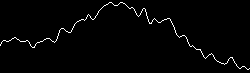
\includegraphics[scale=1.5]{images/plottingsample.png}
\caption[EEG Signal Mapping to Images]{Sample EEG signal plot.  For this sample image, the length of the signal is 1s, which is 250 sample points.  The height of the image is 73 pixels, which is the peak-to-peak amplitude of the signal segment.  Channel Oz of baseline EEG activity is being shown.}
\label{fig:plottingsample}
\end{figure}

This chapter mostly deal with the coordinates transformation that need to be enforced while converting the signal into a plot.  Figure \ref{fig:imagecoordinatesystem} shows the image coordinate system where the $(z_1,z_2)$, with  $z_1,z_2 \in \mathbb{N}^0 \times \mathbb{N}^0$, represent the horizontal and vertical locations, and the $(0,0)$ value is the upper-left position of the image. 

\begin{figure}[h!]
\centering
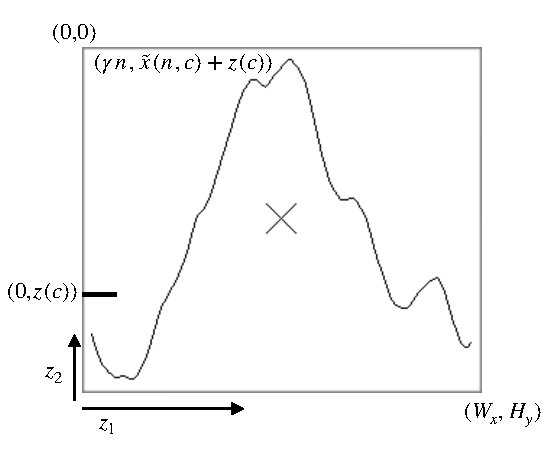
\includegraphics[scale=1.2]{images/imagecoordinatesystem.pdf}
\caption[Image Coordinate System]{The image coordinate system and the mapping from the signal segment.  The origin is the $(0,0)$ position at the upper-left corner of the image.  Time is represented as sample points on the horizontal axis, and the amplitude in $\mu V$ is shown on the vertical axis. Image height $H_y$ and width $W_x$ are obtained based on signal parameters.  The signal's zero-level $z(c)$ is the vertical location where the signal zero value is located. The plot of the signal is obtained by first setting the sample points on the predetermined image locations according to equation \ref{eq:images} and then applying a discrete interpolation algorithm to connect them with straight lines. The plotted waveform is a K-Complex.}
\label{fig:imagecoordinatesystem}
\end{figure}

%\begin{figure}[]
%\centering
%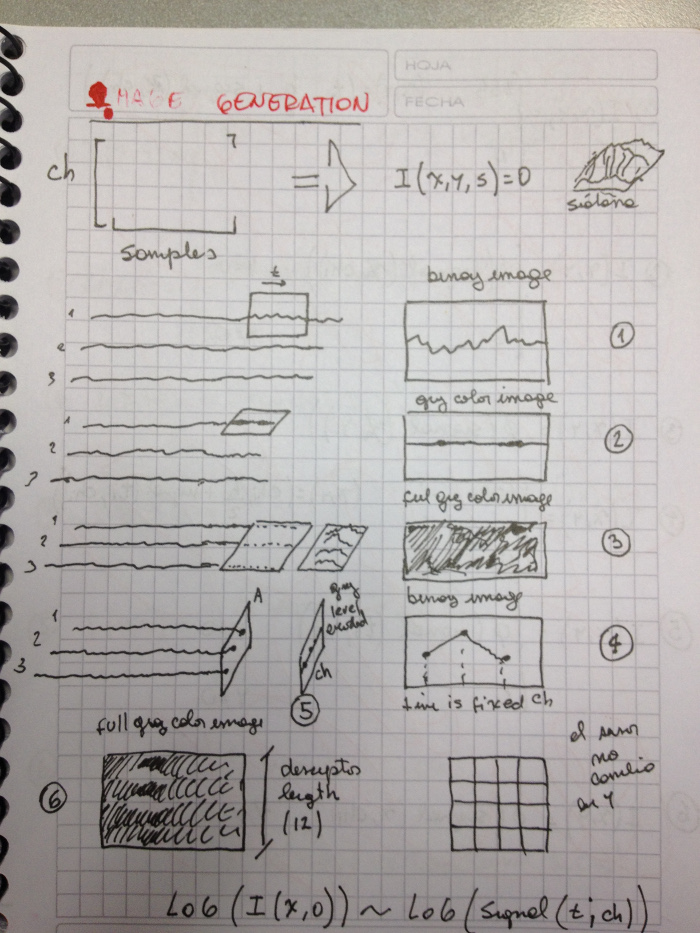
\includegraphics[scale=0.2]{images/SignalTransformation.jpg}
%\caption[EEG Signal Mapping to Images]{Six ways of mapping an EEG signal segment into a binary or greyscale image.}
%\label{fig:mappingimages}
%\end{figure}

Let $c_i$ be a given constant channel, the values of $\mathcal{I}(z_1,z_2)$ are obtained for $n$ varying between $1$ and $N$ or $c$ varying between $1$ and $C$.   In order to convert the EEG original signal $x(n,c)$ into a time-domain image $\mathcal{I}(z_1,z_2)$ representation, the following six alternatives can be used:

\begin{enumerate}
\item Channel-by-channel binary image:

The standard plotting, on a black-and-white image with lines representing voltage amplitude:

\begin{equation}
\mathcal{I}^{(c_i)}(z_1,z_2)= \left\{ \begin{array}{rl}
255 & \text{if} \,  z_1 =  n; \; z_2 = x(n,c_i) + z(c_i) \\
0   & \mbox{otherwise}
\end{array}\right    ..
\label{eq:image1}
\end{equation}

Due to the coordinates transformation, the signal plotted by this procedure is inverted on the image.  Thus, it is necessary to multiply $x(n,c_i)$ by $(-1)$ to invert it before plotting.

\item Channel-by-channel greyscale image

The voltage amplitudes are represented in greyscale, that could range between 0 and 255.  The function $\phi( \cdot )$ is a bounded linear mapping between $\left[ 0,255 \right]$:

\begin{equation}
\mathcal{I}^{(c_i)}(z_1,z_2)= \left\{ \begin{array}{rl}
\phi(x(n,c_i)) & \text{if} \,  z_1 = n; \; z_2 = z(c_i) \\
0   & \mbox{otherwise}
\end{array}\right ..
\label{eq:image2}
\end{equation}

\item Multichannel full greyscale image

The image is greyscale. Voltage amplitudes are represented by the pixel content and each channel is represented on the vertical axis.  The height of the signal is equal to the number of channels.   This is used in Neuroimaging~\cite{Freeman2013} plots of ERP events:

\begin{equation}
\mathcal{I}(z_1,z_2) = \left\{ \begin{array}{rl} \phi(x(n,c))  & \text{if} \,  z_1 = n; \; z_2 = c \end{array}\right. .
\label{eq:image3}
\end{equation}


\item Multichannel stationary binary image:

The horizontal axis of the image is not time, but it is the number of the channel instead.   In this representation different contributions from different channels can be explored at the same time, but time dynamics is lost.  

\begin{equation}
\mathcal{I}^{(n_i)}(z_1,z_2) = \left\{ \begin{array}{rl}
255 & \text{if} \,  z_1 = c; \; z_2 =  x(n_i,c) + \mathtt{Z} \\
0   & \mbox{otherwise}
\end{array}\right ..
\label{eq:image4}
\end{equation}

In this case, the vertical position where the signal's zero value is located in $\mathtt{Z}$.

\item Multichannel stationary greyscale image

This is a variant of the previous one, where the horizontal axis also represent the channel.   In this form, the intensity of the contribution of each channel is represented by the greyscale pixel value.  Combined with head models and forward projection solutions this is the methodology used to represent scalp heatmaps~\cite{Gramfort2013}:

\begin{equation}
\mathcal{I}^{(n_i)}(z_1,z_2)= \left\{ \begin{array}{rl}
\phi(x(n_i,c)) & \text{if} \,  z_1 = c; \; z_2 =  \mathtt{Z} \\
0   & \mbox{otherwise}
\end{array}\right ..
\label{eq:image5}
\end{equation}


\item Channel by channel full greyscale image

This is similar to a raster plot~\cite{Cohen2014} but the greyscale image representing voltages in pixel intensities can be replicated or epoched $H$ times, which at the same time is the height of the image.  The selection of this value depends on the number of epochs or repetitions to show.  In this case, the mapping is

\begin{equation}
\mathcal{I}^{(c_i)}(z_1,z_2) = \left\{ \begin{array}{rl} \phi(x(n,c_i))  & \text{if} \,  z_1 = n; \; z_2 = H \end{array}\right. .
\label{eq:image6}
\end{equation}

%This last representation has the important property that $ LoG(I(x,0)) = LoG(x(n,c)) $.

\end{enumerate}


To analyze effectively an EEG signal, many signal segments must be produced.  Hence, the transformation from signal to image is continuously repeated, and many images need to be crafted for the EEG signal under analysis.  How to determine the size of all the images so that they can be effectively compared between them ?  The first option is to regularize the signal and fit in an equal size for every image.  An alternative choice is to autoscale every image according to the zero-level position.  Figure \ref{fig:plottingscheme} shows two sample artificial impulse signals and their  alternative transformation into images.

%TODO hay un tercero que seria no aplicar el zscore y ajustar el tamanio a la amplitud point to point y poner el keypoint en la mitad de la senial.
\section{Standardized plotting}
\label{standardized}

The \textit{z-score} is a widely used method to regularize a signal~\cite{VandenBerg2006,Zhang2013}. This standardization procedure is defined for  $1 \leq n \leq N$ and $1 \leq c \leq C$ by doing

\begin{equation}
\tilde{x}(n,c) =  \frac{ x(n,c) - \bar{x}(c) }{ \hat{\sigma}(c) } 
\label{eq:standarizedaverages}
\end{equation}

\noindent  where $ x(n,c) $ is the multichannel EEG signal segment for the sample point index $n$ and for channel $c$. The values $$\bar{x}(c) =\frac{1}{N}\sum_{n=1}^{N}x(n,c)$$ and $$ \hat{\sigma}(c) =   \bigg \{ \frac{1}{N-1}\sum_{n=1}^{N} { \left[ x(n,c)-\bar{x}(c) \right]  }^2 \bigg \}^{\frac{1}{2}}$$ are the mean and estimated standard deviation of $x(n,c), 1 \leq n \leq N$, for each channel $c$. Figure~\ref{fig:plottingscheme}(a) shows an impulse signal and their standardized representation.

\section{Autoscaled plotting}
\label{autoscaled}

This plotting scheme allows each image to adapt to the underlying signal.  The signal is centered~\cite{VandenBerg2006} while the image height is autoscaled. The height is set at twice the value of the zero-level, and the signal mean is subtracted from the original signal, producing a vertical displacement, according to the following Equation,

\begin{equation}
\tilde{x}(n,c) =  x(n,c) - \bar{x}(c) 
\label{eq:autoscaled}
\end{equation}

Figure \ref{fig:plottingscheme}(b) shows the results of the plotting for an impulse signal.  Equation~\ref{eq:autoscaled} has the advantage that any low frequency component, particularly the EEG DC drift is eliminated, due to the fact that plot of the signal is always centered on each image.

\begin{figure}[htb]
\centering
\subfigure[Standardized: The signal is standardized and the height of the image is determined according to the peak-to-peak amplitude, which is similar for every image.]
{
\includegraphics[height=5cm,width=7.5cm]{images/standardized.eps}}
\subfigure[Autoscaled: The plotted image height is twice the zero-level, which is also determined according to the peak-to-peak amplitude of each segment, proportional to $\gamma$, and not constant. Transformed images do not have the same height, but the zero-level is always located at half the height of the image.]
{
\includegraphics[height=5cm,width=7.5cm]{images/autoscaled.eps}}
\caption[Signal plotting schemes]{An artificial signal pulse and its plotting representations.}
\label{fig:plottingscheme}
\end{figure}

\section{Zero-Level}

The zero-level $z(c)$ is the image vertical position where the signal's zero value has to be situated in order to fit the entire signal within the image for each channel c:

\begin{equation}
z(c) = \left \lfloor{ \frac{\max_{n} \tilde{x}(n,c)  - \min_{n} \tilde{x}(n,c) }{2} }\right \rfloor -   \left \lfloor{ \frac{\max_{n} \tilde{x}(n,c)  + \min_{n} \tilde{x}(n,c)}{ 2} }\right \rfloor
\label{eq:zerolevel}
\end{equation}

\noindent where the minimization and maximization are carried out for $n$ varying between ${1 \leq n\leq N}$. This value represents the vertical location on the image where the signal goes to zero.  

\section{Image Size}

\subsubsection{Height}

The height of the image is calculated according to the peak-to-peak amplitude of the signal segment, and proportional to the amplitude scale factor $\gls{gamma}$:

\begin{equation}
H_y = \max \left\lfloor \gamma \; \tilde{x}(n,c) \right\rceil  - \min \left\lfloor \gamma \; \tilde{x}(n,c) \right\rceil 
\label{eq:height}
\end{equation}

\noindent while for the autoscalable version, it is just twice the value of the zero-level:

\begin{equation}
H_y = 2 \; z(c) .
\label{eq:autoscaleheight}
\end{equation}


\subsubsection{Width}

The width, on the other hand, is obtained based on the length of the signal segment, scaled by the $\gamma_t$  time factor,

\begin{equation}
W_x = \gamma_t  N
\label{eq:width}
\end{equation}

\section{EEG Signal Plot}
\label{Plot}

Once the regularization procedure,  the size and the scale of the image are defined,  a binary image $\mathcal{I}^{(c)}$ can be constructed from a variant of the method specified in Equation~\ref{eq:image1} according to

\begin{equation}
\mathcal{I}^{(c)}(z_1,z_2) = \left\{ \begin{array}{rl}
255 & \text{if} \   z_1 = \gamma_{t} \  n \quad \text{and}  \quad z_2 = \left\lfloor \gamma \; \tilde{x}(n,c) \right\rceil + z(c) \\
0   & \mbox{otherwise}
\end{array}\right.
\label{eq:images}
\end{equation}

\noindent  where  $1 \leq c \leq C$ and $1 \leq n \leq N$. The amplitude scale factor $\gls{gamma}$ and time scale factor $\gls{gammat}$ are used to determine the image size and at the same time the image resolution. This scheme produces a black-and-white plot of the signal with $255$ being white and $0$ black.  There is one image per channel per segment. 

%\noindent with $255$ being white and representing the signal's voltage in relation to the zero-level $z(c)$, and $0$ for black which is the background contrast. This scheme produces a black-and-white plot of the signal.  Pixel arguments $ (z_1,z_2) \in \mathbb{N} \times \mathbb{N}$ iterate over the width $\gls{Wx}$ and height $\gls{Hy}$  of the image plot with $1 \leq n \leq N$ and $1 \leq c \leq C$.  There is one image per channel.  The parameters $\gamma$ and $\gamma_t$ are the amplitude and time scaling factors.  They are used to determine the image size and at the same time the image resolution.

\section{Interpolation}

Equation \ref{eq:images} produces a set of isolated pixels over the image $\mathcal{I}^{(c)}$.  To produce the plot $I^{(c)}$, the Bresenham \cite{Bresenham1965,Ramele2016} algorithm is used to digitally interpolate straight lines between each pair of consecutive pixels.  Figure~\ref{fig:interpolation}(a) shows an image plot constructed by only using the sample points, while~\ref{fig:interpolation}(b) shows the digital interpolation produced by the Bresenham algorithm.

\begin{figure}[h!]
\centering
\subfigure[Sample points are located on the image according to Equation \ref{eq:images}. ]
{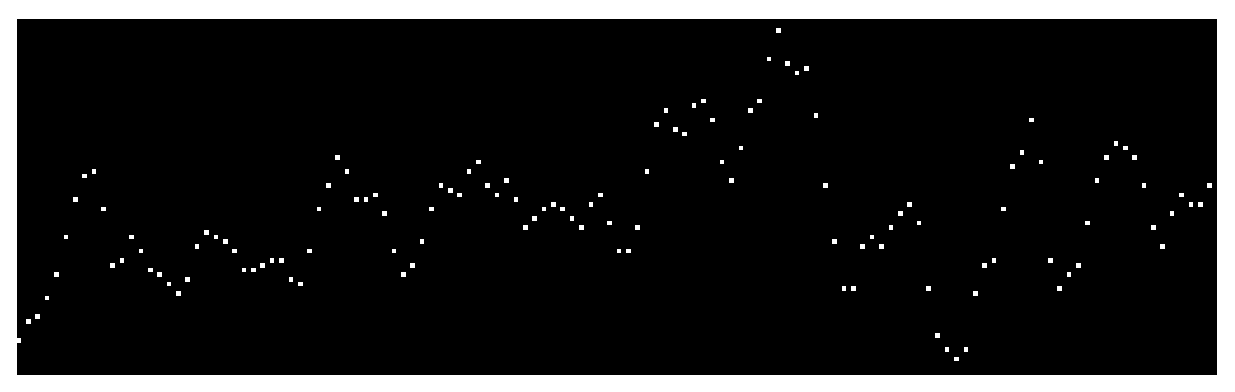
\includegraphics[height=4cm,width=15cm]{images/samplepoints.eps}}
\subfigure[Sample points are linearly interpolated in a discrete procedure using the Bresenham algorithm.]
{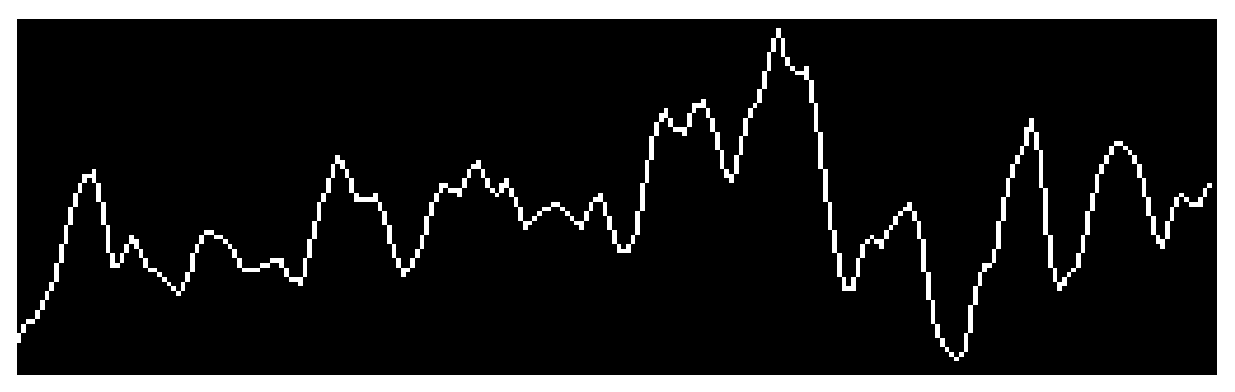
\includegraphics[height=4cm,width=15cm]{images/bresenham.eps}}
\subfigure[The digital signal is scaled 4 times ($\gamma_t=4$) and the generated sample points are interpolated using the Bresenham algorithm.]
{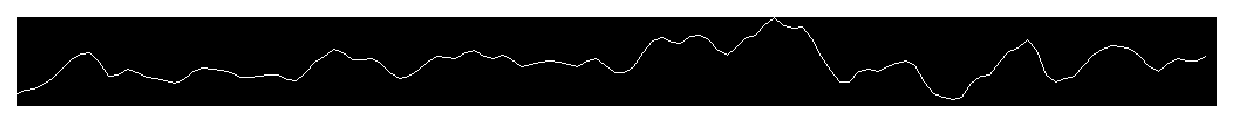
\includegraphics[height=4cm,width=15cm]{images/upscaled.eps}}
\subfigure[The digital signal is upsampled 4 times with a linear interpolation with splines. The Bresenham algorithm is used to perform the final digital interpolation to compose the plot.]
{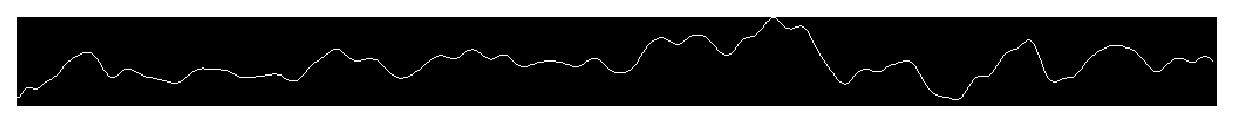
\includegraphics[height=4cm,width=15cm]{images/upsample.eps}}
\caption[Signal Plotting: Interpolation]{Generated images based on different interpolation schemes.}
\label{fig:interpolation}
\end{figure}

On Figure~\ref{fig:interpolation}(c) the same signal can be observed produced when the time scaling factor $\gls{gammat}$ is increased to $4$. It can be noticed that there are very sharp edges around sample pixels.  This can lead to a quantization of histogram gradients that will be discussed in the next Chapter. To reduce this sharpness of the signal on the plot, an alternative procedure is to use a smoothing interpolation of the signal $\tilde{x}(n,c)$ using splines.  Instead of just situating time point values at a bigger step according to Equation~\ref{eq:images}, intermediate values are computed according to a linear, quadratic or cubic interpolation, hence smoothing the curve around each point.  The result of this interpolation can be seen on Figure~\ref{fig:interpolation}(d), where the edges around each sample point are more rounded. This procedure is similar to what the Matlab's \textbf{resample} function does which also includes an antialiasing FIR lowpass filter~\cite{Oppenheim2009}.

Special care must be taken by the presence of artifacts around the signal endpoints, at the edges of the image. Those regions are excluded from further analysis.

\begin{figure}[htb]
\centering
\subfigure[Vertical axis is voltage in $\mu V$ while horizontal axis is expressed in sample points units.]
{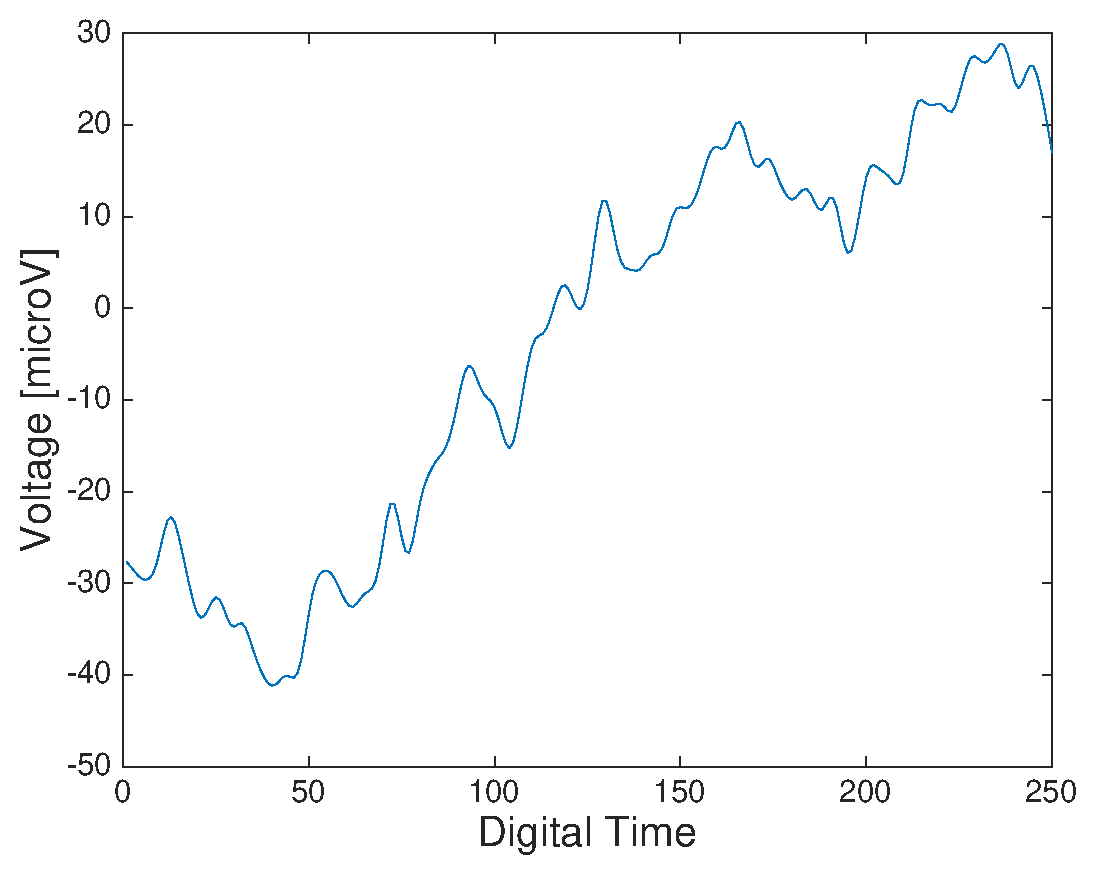
\includegraphics[height=5cm,width=5cm]{images/plotvsimage.eps}}
\subfigure[An image generated by the plotting algorithm for the same signal. Image height is $76$ pixels, while width is $250$. The zero-level $z(c)$ value is $32$.]
{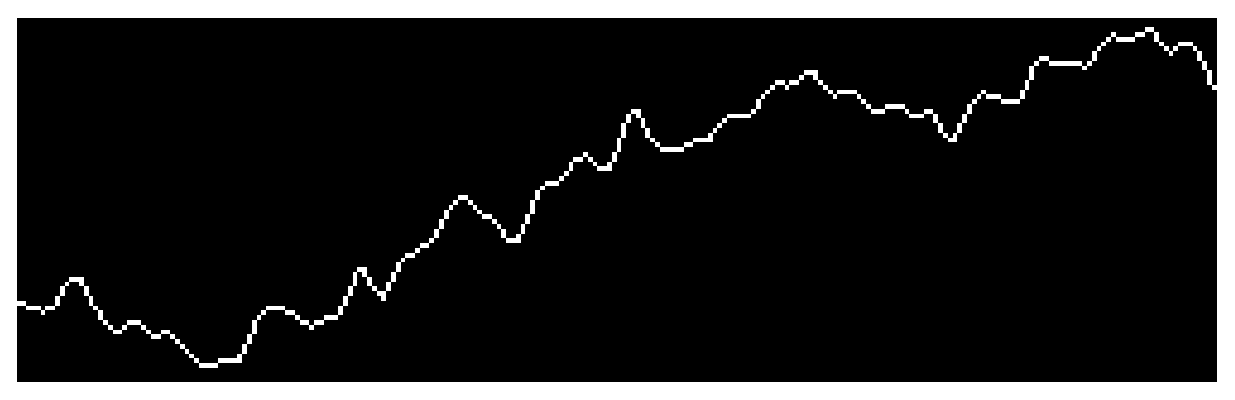
\includegraphics[height=5cm,width=10cm]{images/sampleplot.eps}}
\caption[Signal and Plot]{One-second length basal EEG signal and the generated image, with $\gls{Fs} = 250$. }
\label{fig:plotvsimage}
\end{figure}

\section{Resolution and Precision}

Image creation and signal plotting is a digitalization process~\cite{Schomer2010}.  Figure~\ref{fig:plotvsimage} shows an EEG signal and their plot representation.  Any digitalization process is defined by their resolution, precision and dynamic range.

The resolution~\cite{Cohen2014} of the image transformation can be determined based on the characteristics of the digital signal and the parameter selection. On the horizontal axis of the image, one pixel is equivalent to 

\begin{equation}
1 P_x \equiv \frac{1}{F_s  \; \gamma_t}  [\si{s}]
\label{eq:resolutionx}
\end{equation}

\noindent where $\gls{Fs}$ is the sampling frequency in Hertz, and $\gls{gammat}$ is the time scale factor.  This gives a value in seconds.  For example, for Figure \ref{fig:plottingsample} where the length is $1 s$, the sampling frequency is $250 Hz$, and $\gls{gammat}= 1$, this gives a resolution of $1 P_x \equiv 0.0040 \si{s}$. Table~\ref{tab:precisionx} shows some reference values.

\begin{table}[htb]
\caption[Reference Values for Horizontal Resolution]{Reference values for horizontal resolution}
\centering
\vspace{8pt}
%% \tablesize{} %% You can specify the fontsize here, e.g.  \tablesize{\footnotesize}. If commented out \small will be used.
\begin{tabular}{|c|c|}
\toprule
\textbf{$\gamma_t$}	&  $1 P_x$  \\
\midrule
 1    &     $1 \; \frac{1}{\gls{Fs}} \si{s}$    \\
 2    &     $\frac{1}{2} \; \frac{1}{\gls{Fs}} \si{s}$    \\
 3    &     $\frac{1}{3} \;  \frac{1}{\gls{Fs}} \si{s}$    \\
 10   &     $\frac{1}{10} \; \frac{1}{\gls{Fs}} \si{s}$    \\
 100 &     $\frac{1}{100} \; \frac{1}{\gls{Fs}} \si{s}$    \\
\bottomrule
\end{tabular}
\label{tab:precisionx}
\end{table}

Consistently, on the vertical axis, one pixel is analogous to 

\begin{equation}
1 P_y \equiv \frac{1}{\gamma}  [\si\mu{V}]
\label{eq:resolutiony}
\end{equation}

\noindent where $\gamma$ is the amplitude scale factor.  As EEG time-series are digitalized in $\si\mu{V}$, this is the unit of choice.  In Figure \ref{fig:plottingsample}, $1$ vertical pixel represents exactly $1 \mu V$.  It is important to notice that the minimum recommended resolution for an EEG device is around $0.5$ $\mu V$, which is an acceptable and practical level to detect physiological meaningful signals~\cite{Schomer2010}.  This level can be reached when $\gls{gamma}$ is equal to $2$.  See Table~\ref{tab:precisiony} to see some reference values.

\begin{table}[htb]
\caption[Reference Values for Vertical Precision and Resolution]{Reference values for vertical precision and resolution}
\centering
\vspace{8pt}
%% \tablesize{} %% You can specify the fontsize here, e.g.  \tablesize{\footnotesize}. If commented out \small will be used.
\begin{tabular}{|c|c|c|}
\toprule
\textbf{$\gamma$}	&  $1 P_y$ 	&  Decimal Precision   \\
\midrule
1     &     $1 \si\mu{V}$   &  $0$                                      \\
2    &     $\frac{1}{2} \si\mu{V}$   &  $0.5$         \\
3     &     $\frac{1}{3} \si\mu{V}$   &  $0.3$   \\
10     &     $\frac{1}{10} \si\mu{V}$   &  $0.1$         \\
100     &     $\frac{1}{100} \si\mu{V}$   &  $0.01$    \\
\bottomrule
\end{tabular}
\label{tab:precisiony}
\end{table}

Regarding the \textit{precision}, discrete EEG time-series are floating-point numbers and the image is constructed based on discrete and integer pixels.  Image's pixel values $(z_1,z_2)$ are obtained according to Equation~\ref{eq:images}.  Thus, on the horizontal axis $z_1$, no discretization is needed because time is already digitalized in sample units. Hence, there is no loss of precision in time from the one generated by the digital device where pixel values are obtained with

\begin{equation}
z_1 = \gamma_t  \; n,
\label{eq:horizontalpixelation}
\end{equation}

\noindent where $n$ refer to the sample point index. The maximum frequency that can be captured by the plotting scheme is half the number of pixels per seconds~\cite{Schomer2010}.  Equation~\ref{eq:horizontalpixelation} determines at least a $1$-to-$1$ relationship between pixels and sample points, thus the effective maximum frequency is only constrained by the Nyquist Frequency~\cite{Oppenheim2009}. 

On the other hand, on the vertical axis, pixels are discretized according to

\begin{equation}
z_2 = \left \lfloor{ \gamma  \; \tilde{x}(n,c)  }\right \rceil
\label{eq:verticalpixelation}
\end{equation}

\noindent where $\gamma$ is the amplitude scale factor parameter, which also affects the height of the image in Equation \ref{eq:height}. A rounding operation $\lfloor  \cdot \rceil$ is applied to obtain an integer representation.  This means that precision is lost on the voltage amplitude.  Table~\ref{tab:precisiony} shows some decimal precision values for different $\gls{gamma}$.

Finally, the dynamic range of the digital capturing device is reduced to what is actually needed for each segment, because the height of the image is adjusted dynamically to the peak-to-peak amplitude, regardless of the plotting scheme.



